\documentclass[journal]{IEEEtai}

\usepackage[colorlinks,urlcolor=blue,linkcolor=blue,citecolor=blue]{hyperref}

\usepackage{color,array}

\usepackage{graphicx}

%% \jvol{XX}
%% \jnum{XX}
%% \paper{1234567}
%% \pubyear{2020}
%% \publisheddate{xxxx 00, 0000}
%% \currentdate{xxxx 00, 0000}
%% \doiinfo{TQE.2020.Doi Number}

\newtheorem{theorem}{Theorem}
\newtheorem{lemma}{Lemma}
\setcounter{page}{1}
%% \setcounter{secnumdepth}{0}


\begin{document}


\title{Generative AI and the Riemann zeta zero distribution} 


\author{Placeholder, for double blind review
\thanks{This paragraph of the first footnote will contain the date on which you submitted your paper for review. It will also contain support information, including sponsor and financial support acknowledgment. For example, ``This work was supported in part by the U.S. Department of Commerce under Grant BS123456.'' }
\thanks{Placeholder, for double blind review}
\thanks{This paragraph will include the Associate Editor who handled your paper.}}

\markboth{Journal of IEEE Transactions on Artificial Intelligence, Vol. 00, No. 0, Month 2020}
{First A. Author \MakeLowercase{\textit{et al.}}: Bare Demo of IEEEtai.cls for IEEE Journals of IEEE Transactions on Artificial Intelligence}

\maketitle

\begin{abstract}
The Transformer model of Generative AI introduced attention mechanisms that has had important successes in natural language processing.  We applied it for predicting the distribution of Riemann zeta zero counts on consecutive Gram intervals. The results are very good. We get accuracies of $0.998$ in predicting a sequence of ten consecutive zero counts. The input for the prediction is a sequence of the preceeding ten zero counts on sequential Gram intervals. We tested with two ranges of Riemann zeta zeros, t (height along critical axis for Riemann zeta function) = $10^{12}$ and t = $10^{28}$. The $0.998$ comes about because the intervals with $3$ or more zeros are rare. With special training for rare events, we can get essentially completely accurate prediction. One surprising result is that the model trained on a small amount of data at $10^{28}$ accurately predicts the behaviour $16$ orders of magnitude away, at $10^{12}$. The high prediction accuracy was unexpected. We present arguments that the 100\% accurate predictions cannot continue indefinitely. Our study shows that applying the technique to more complex problems has great promise. We have used very minimal computer resources compared to typical models in language applications. With access to better resources, we can attack much more important problems. 
\end{abstract}

\begin{IEEEImpStatement}
Our application of the Transformer model, renowned for its attention mechanisms in natural language processing, marks a significant breakthrough in predicting the distribution of Riemann zeta zero counts on consecutive Gram intervals. Achieving accuracies as high as $0.998$ in forecasting sequences of ten consecutive zero counts underscores the model's robustness and effectiveness in this specialized domain. By focusing on rare events — intervals with three or more zeros — and employing tailored training strategies, we achieved near-perfect predictions, showcasing the Transformer's adaptability beyond traditional linguistic tasks. Moreover, our study demonstrates promising potential for applying these techniques to more intricate problems, leveraging minimal computational resources compared to standard language models. With enhanced computational capabilities, we anticipate tackling even more impactful challenges, highlighting the transformative impact of advanced AI methodologies in mathematical research and beyond.

\end{IEEEImpStatement}

\begin{IEEEkeywords}
Enter key words or phrases in alphabetical order, separated by commas. For a list of suggested keywords, send a blank e-mail to \href{mailto:keywords@ieee.org}{\underline{keywords@ieee.org}} or visit \href{http://www.ieee.org/organizations/pubs/ani_prod/keywrd98.txt}{\underline{http://www.ieee.org/organizations/pubs/ani\_prod/keywrd98.txt}}
\end{IEEEkeywords}



\section{Introduction}

\IEEEPARstart{T}{he}  Transformer model~\cite{vaswani2017attention} introduced attention mechanisms that revolutionized natural language processing.
Recent advancements \cite{radford2019language} and \cite{brown2020language} include significant improvements in few-shot learning capabilities.
The effectiveness of transfer learning using a unified text-to-text Transformer approach. is studied in \cite{raffel2019exploring}.
Transformer-XL, described in \cite{dai2019transformerxl}, extends the Transformer architecture to handle longer contexts in language modeling tasks.
Transformer-XH, proposed by \cite{zhang2019transformerxh}, addresses multi-hop question answering with explanation capabilities.


\section{Background}

xxx

\subsection{Abbreviations and Acronyms}

Define 


\section{Methodology}

If 

\subsection{Equations}
xxx

\section{Theory/Analysis}

Use 


\begin{figure}
\centerline{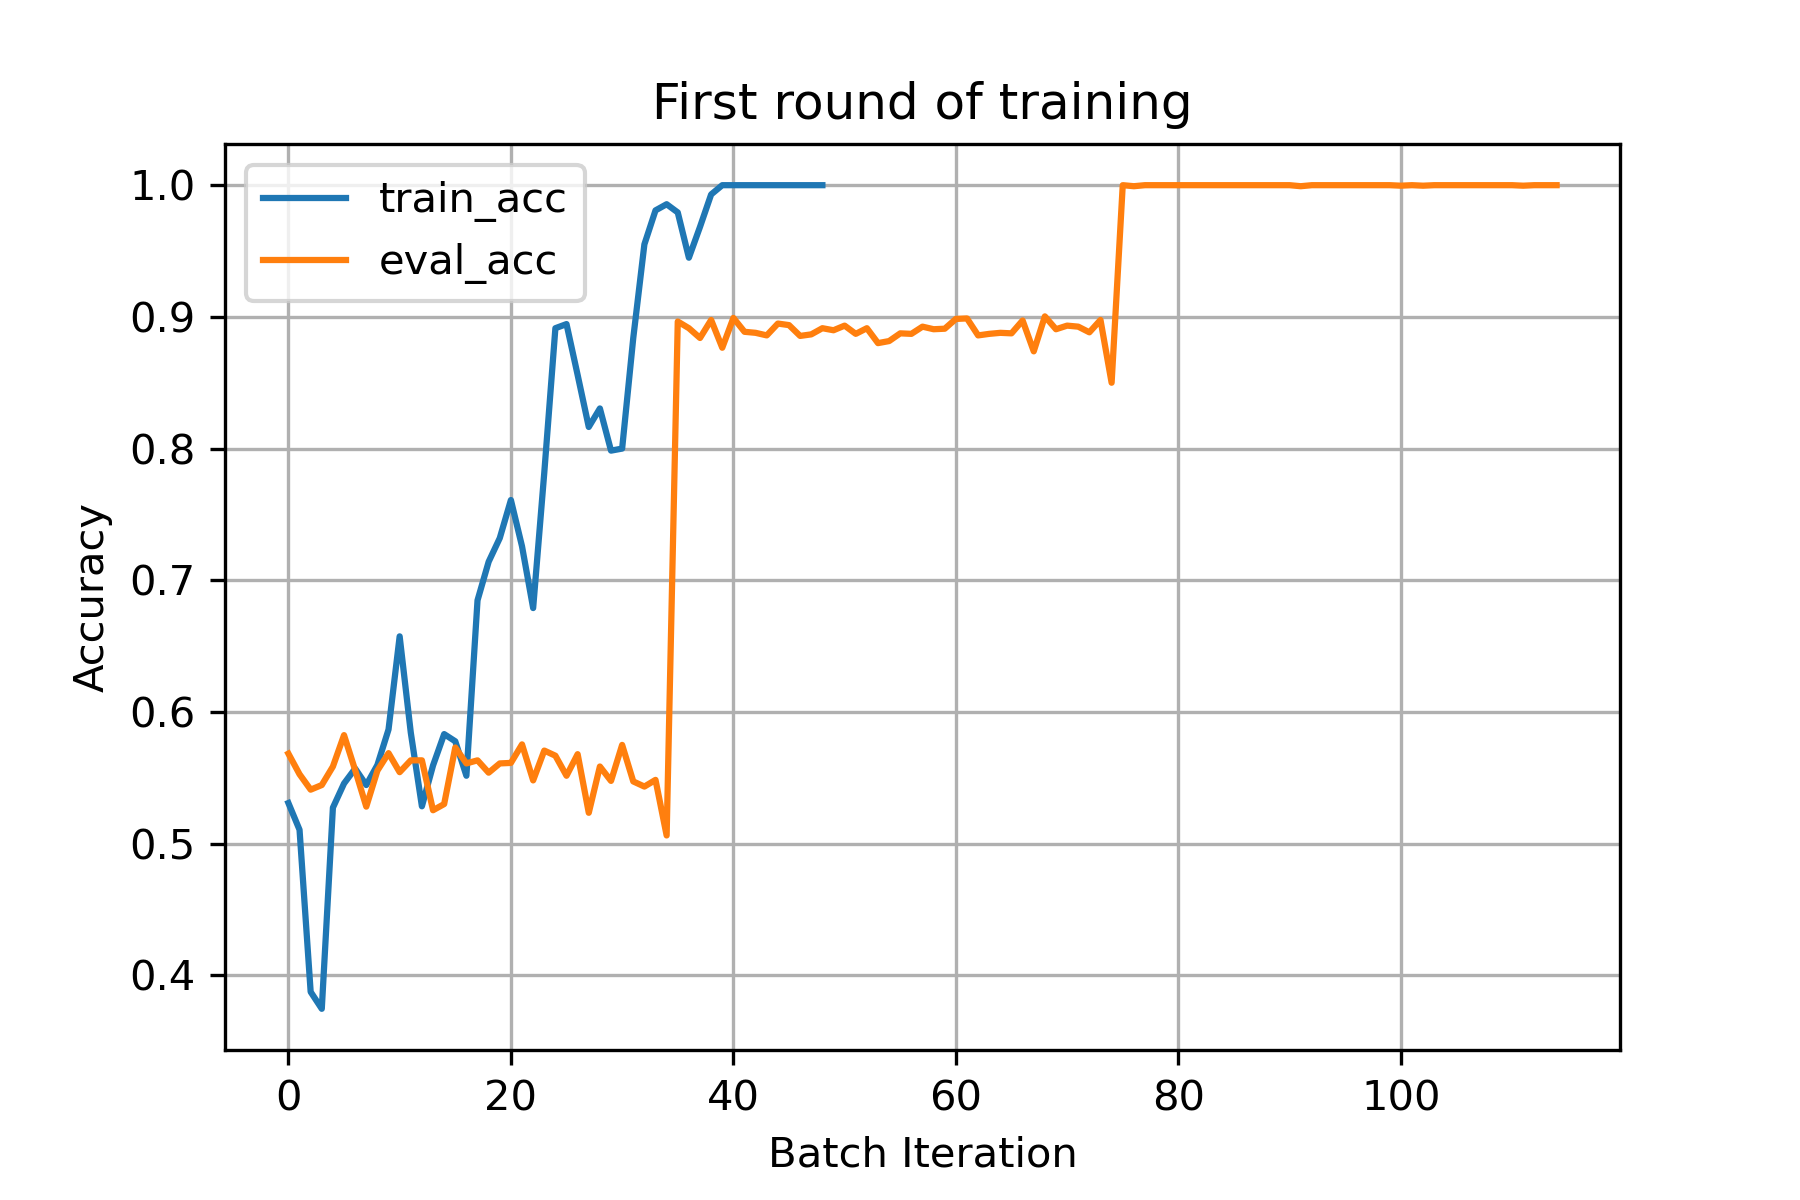
\includegraphics[width=18.5pc]{Figure1.png}}
\caption{Magnetization as a function of applied field. Note that ``Fig.'' is abbreviated. There is a period after the figure number, followed by two spaces. It is good practice to explain the significance of the figure in the caption.}
\end{figure}




\section{Conclusion and Future Work}

A conclusion section is not required. Although a conclusion may review the main points of the paper, do not replicate the abstract as the conclusion. A conclusion might elaborate on the importance of the work or suggest applications and extensions.






\section*{References}

\begin{thebibliography}{34}

\bibitem{vaswani2017attention}
A. Vaswani, N. Shazeer, N. Parmar, J. Uszkoreit, L. Jones, A. N. Gomez, Ł. Kaiser, and I. Polosukhin, "Attention is all you need," in \emph{Advances in Neural Information Processing Systems (NeurIPS)}, vol. 30, 2017, pp. 5998--6008.

\bibitem{radford2019language}
A. Radford, J. Wu, R. Child, D. Luan, D. Amodei, and I. Sutskever, "Language models are unsupervised multitask learners," \emph{OpenAI Blog}, vol. 1, no. 8, 2019, p. 9.

\bibitem{brown2020language}
T. B. Brown, B. Mann, N. Ryder, M. Subbiah, J. Kaplan, P. Dhariwal, A. Neelakantan, P. Shyam, G. Sastry, A. Askell, et al., "Language models are few-shot learners," in \emph{Advances in Neural Information Processing Systems (NeurIPS)}, vol. 33, 2020.

\bibitem{raffel2019exploring}
C. Raffel, N. Shazeer, A. Roberts, K. Lee, S. Narang, M. Matena, Y. Zhou, W. Li, and P. J. Liu, "Exploring the limits of transfer learning with a unified text-to-text transformer," \emph{arXiv preprint arXiv:1910.10683}, 2019.

\bibitem{dai2019transformerxl}
Z. Dai, Z. Yang, Y. Yang, J. Carbonell, Q. V. Le, and R. Salakhutdinov, "Transformer-XL: Attentive language models beyond a fixed-length context," in \emph{Proceedings of the 57th Annual Meeting of the Association for Computational Linguistics (ACL)}, 2019, pp. 2978--2988.

\bibitem{zhang2019transformerxh}
Y. Zhang, Z. Gan, R. Henao, D. Shen, and L. Carin, "Transformer-XH: Multi-hop question answering with explanation," in \emph{Advances in Neural Information Processing Systems (NeurIPS)}, vol. 32, 2019.

\end{thebibliography}






\begin{IEEEbiography}{First A. Author}{\space}   placeholder, for double blind review
\end{IEEEbiography}


\end{document}
